% Created by tikzDevice version 0.8.1 on 2015-01-12 17:01:40
% !TEX encoding = UTF-8 Unicode
% Calculated string width of 0.00 as 17.062600
% Calculated character metrics. ascent: 6.611760, descent: 0.000000, width: 8.797910
% Calculated string width of 0.05 as 17.062600
% Calculated string width of 0.10 as 17.062600
% Calculated string width of 0.15 as 17.062600
% Calculated string width of 0.20 as 17.062600
% Calculated string width of 0.00 as 17.062600
% Calculated string width of 0.05 as 17.062600
% Calculated string width of 0.10 as 17.062600
% Calculated string width of 0.15 as 17.062600
% Calculated string width of 0.20 as 17.062600
% Calculated string width of -10 to -6 as 35.724850
% Calculated string width of -5 to 0 as 27.726750
% Calculated string width of 1 to 5 as 24.527510
% Calculated string width of 6 to 10 as 29.326370
% Calculated string width of 0.00 as 17.062600
% Calculated string width of 0.25 as 17.062600
% Calculated string width of 0.50 as 17.062600
% Calculated string width of 0.75 as 17.062600
% Calculated string width of 1.00 as 17.062600
% Calculated string width of 0.00 as 17.062600
% Calculated string width of 0.25 as 17.062600
% Calculated string width of 0.50 as 17.062600
% Calculated string width of 0.75 as 17.062600
% Calculated string width of 1.00 as 17.062600
% Calculated string width of Proportion as 57.219210
% Calculated character metrics. ascent: 8.264620, descent: 0.000000, width: 10.997280
% Calculated string width of Estimated Probability as 116.404600
% Calculated string width of Proportion as 57.219210
% Calculated string width of Estimated Probability as 116.404600
% Drawing Rectangle from x0 = 0.000000, y0 = 0.000000 to x1 = 505.890000, y1 = 361.350000
% Beginning new tikzpicture 'page'
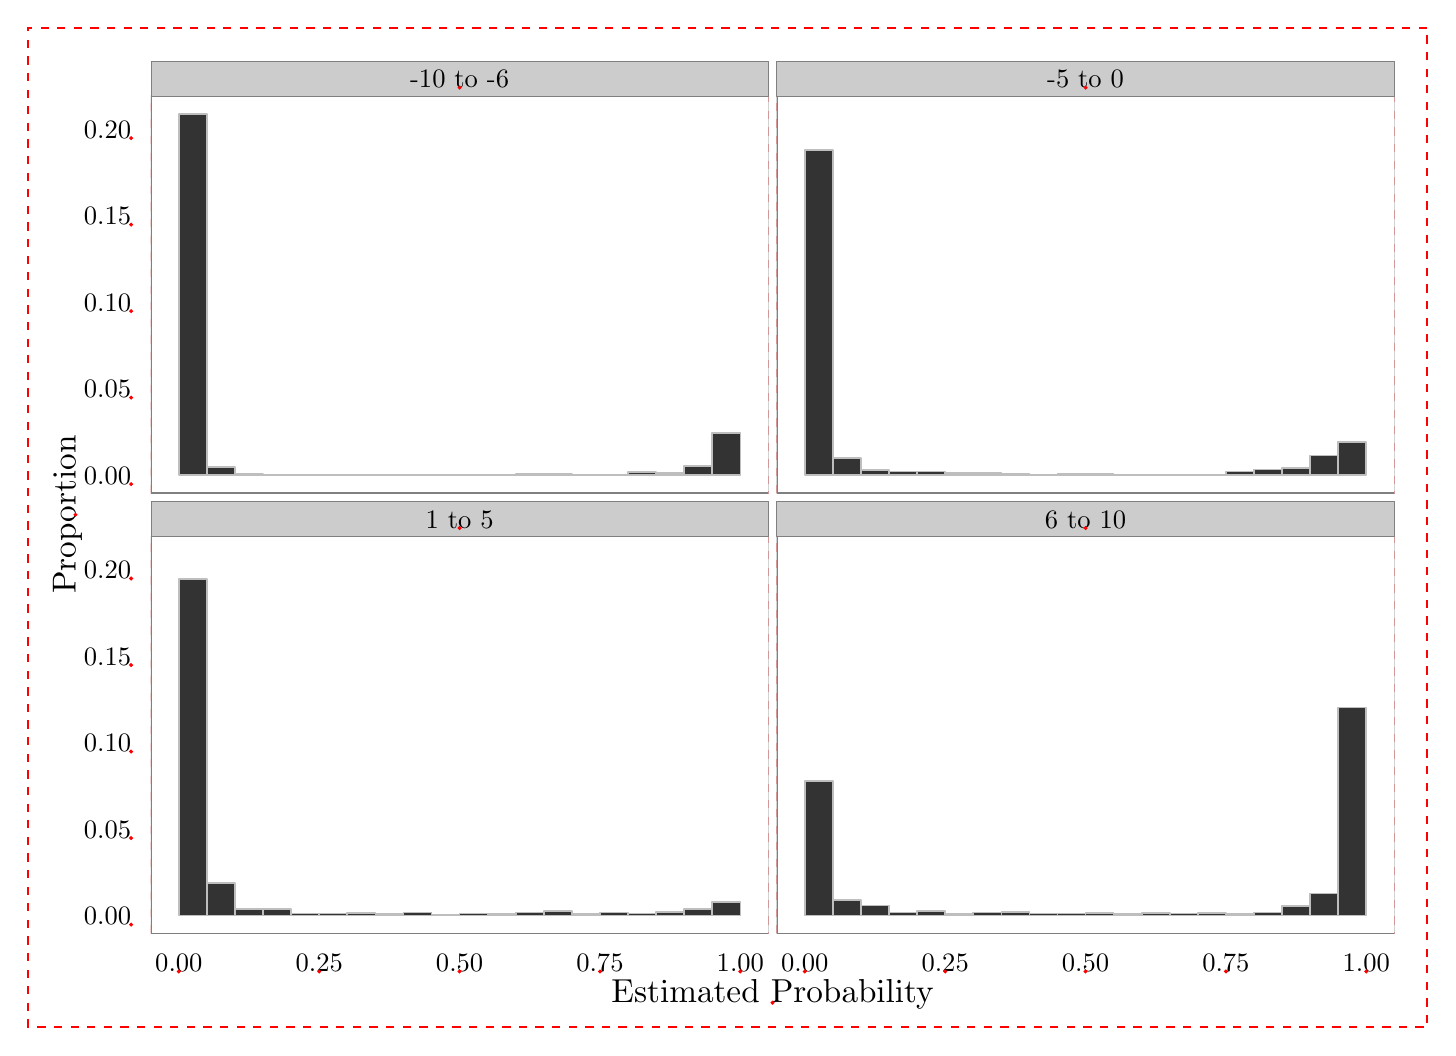
\begin{tikzpicture}[x=1pt,y=1pt]
\definecolor{fillColor}{RGB}{255,255,255}
\path[use as bounding box,fill=fillColor,fill opacity=0.00] (0,0) rectangle (505.89,361.35);
\begin{scope}
\path[clip] (  0.00,  0.00) rectangle (505.89,361.35);
\path[draw=red,very thick,dashed] (  0.00,  0.00) rectangle (505.89,361.35);
\definecolor{drawColor}{RGB}{255,255,255}
\definecolor{fillColor}{RGB}{255,255,255}

\path[draw=drawColor,line width= 0.6pt,line join=round,line cap=round,fill=fillColor] (  0.00,  0.00) rectangle (505.89,361.35);
\end{scope}
% Drawing Rectangle from x0 = 44.485409, y0 = 193.175409 to x1 = 267.659579, y1 = 336.670740
\begin{scope}
\path[clip] ( 44.49,193.18) rectangle (267.66,336.67);
\path[draw=red,very thick,dashed] ( 44.49,193.18) rectangle (267.66,336.67);
\definecolor{fillColor}{RGB}{255,255,255}

\path[fill=fillColor] ( 44.49,193.18) rectangle (267.66,336.67);
% Drawing Rectangle from x0 = 54.629689, y0 = 199.697925 to x1 = 64.773970, y1 = 330.148225
\definecolor{drawColor}{RGB}{190,190,190}
\definecolor{fillColor}{gray}{0.20}

\path[draw=drawColor,line width= 0.6pt,line join=round,fill=fillColor] ( 54.63,199.70) rectangle ( 64.77,330.15);
% Drawing Rectangle from x0 = 64.773970, y0 = 199.697925 to x1 = 74.918250, y1 = 202.572253

\path[draw=drawColor,line width= 0.6pt,line join=round,fill=fillColor] ( 64.77,199.70) rectangle ( 74.92,202.57);
% Drawing Rectangle from x0 = 74.918250, y0 = 199.697925 to x1 = 85.062531, y1 = 200.140129

\path[draw=drawColor,line width= 0.6pt,line join=round,fill=fillColor] ( 74.92,199.70) rectangle ( 85.06,200.14);
% Drawing Rectangle from x0 = 85.062531, y0 = 199.697925 to x1 = 95.206811, y1 = 199.919027

\path[draw=drawColor,line width= 0.6pt,line join=round,fill=fillColor] ( 85.06,199.70) rectangle ( 95.21,199.92);
% Drawing Rectangle from x0 = 95.206811, y0 = 199.697925 to x1 = 105.351092, y1 = 199.697925

\path[draw=drawColor,line width= 0.6pt,line join=round,fill=fillColor] ( 95.21,199.70) rectangle (105.35,199.70);
% Drawing Rectangle from x0 = 105.351092, y0 = 199.697925 to x1 = 115.495372, y1 = 199.697925

\path[draw=drawColor,line width= 0.6pt,line join=round,fill=fillColor] (105.35,199.70) rectangle (115.50,199.70);
% Drawing Rectangle from x0 = 115.495372, y0 = 199.697925 to x1 = 125.639653, y1 = 199.919027

\path[draw=drawColor,line width= 0.6pt,line join=round,fill=fillColor] (115.50,199.70) rectangle (125.64,199.92);
% Drawing Rectangle from x0 = 125.639653, y0 = 199.697925 to x1 = 135.783933, y1 = 199.919027

\path[draw=drawColor,line width= 0.6pt,line join=round,fill=fillColor] (125.64,199.70) rectangle (135.78,199.92);
% Drawing Rectangle from x0 = 135.783933, y0 = 199.697925 to x1 = 145.928214, y1 = 199.919027

\path[draw=drawColor,line width= 0.6pt,line join=round,fill=fillColor] (135.78,199.70) rectangle (145.93,199.92);
% Drawing Rectangle from x0 = 145.928214, y0 = 199.697925 to x1 = 156.072494, y1 = 199.919027

\path[draw=drawColor,line width= 0.6pt,line join=round,fill=fillColor] (145.93,199.70) rectangle (156.07,199.92);
% Drawing Rectangle from x0 = 156.072494, y0 = 199.697925 to x1 = 166.216775, y1 = 199.697925

\path[draw=drawColor,line width= 0.6pt,line join=round,fill=fillColor] (156.07,199.70) rectangle (166.22,199.70);
% Drawing Rectangle from x0 = 166.216775, y0 = 199.697925 to x1 = 176.361055, y1 = 199.697925

\path[draw=drawColor,line width= 0.6pt,line join=round,fill=fillColor] (166.22,199.70) rectangle (176.36,199.70);
% Drawing Rectangle from x0 = 176.361055, y0 = 199.697925 to x1 = 186.505336, y1 = 200.140129

\path[draw=drawColor,line width= 0.6pt,line join=round,fill=fillColor] (176.36,199.70) rectangle (186.51,200.14);
% Drawing Rectangle from x0 = 186.505336, y0 = 199.697925 to x1 = 196.649616, y1 = 200.140129

\path[draw=drawColor,line width= 0.6pt,line join=round,fill=fillColor] (186.51,199.70) rectangle (196.65,200.14);
% Drawing Rectangle from x0 = 196.649616, y0 = 199.697925 to x1 = 206.793897, y1 = 199.697925

\path[draw=drawColor,line width= 0.6pt,line join=round,fill=fillColor] (196.65,199.70) rectangle (206.79,199.70);
% Drawing Rectangle from x0 = 206.793897, y0 = 199.697925 to x1 = 216.938177, y1 = 199.919027

\path[draw=drawColor,line width= 0.6pt,line join=round,fill=fillColor] (206.79,199.70) rectangle (216.94,199.92);
% Drawing Rectangle from x0 = 216.938177, y0 = 199.697925 to x1 = 227.082458, y1 = 200.803436

\path[draw=drawColor,line width= 0.6pt,line join=round,fill=fillColor] (216.94,199.70) rectangle (227.08,200.80);
% Drawing Rectangle from x0 = 227.082458, y0 = 199.697925 to x1 = 237.226738, y1 = 200.361231

\path[draw=drawColor,line width= 0.6pt,line join=round,fill=fillColor] (227.08,199.70) rectangle (237.23,200.36);
% Drawing Rectangle from x0 = 237.226738, y0 = 199.697925 to x1 = 247.371019, y1 = 203.014458

\path[draw=drawColor,line width= 0.6pt,line join=round,fill=fillColor] (237.23,199.70) rectangle (247.37,203.01);
% Drawing Rectangle from x0 = 247.371019, y0 = 199.697925 to x1 = 257.515299, y1 = 214.953977

\path[draw=drawColor,line width= 0.6pt,line join=round,fill=fillColor] (247.37,199.70) rectangle (257.52,214.95);
% Drawing Rectangle from x0 = 44.485409, y0 = 193.175409 to x1 = 267.659579, y1 = 336.670740
\definecolor{drawColor}{gray}{0.50}

\path[draw=drawColor,line width= 0.6pt,line join=round,line cap=round] ( 44.49,193.18) rectangle (267.66,336.67);
\end{scope}
% Drawing Rectangle from x0 = 270.670829, y0 = 193.175409 to x1 = 493.845000, y1 = 336.670740
\begin{scope}
\path[clip] (270.67,193.18) rectangle (493.85,336.67);
\path[draw=red,very thick,dashed] (270.67,193.18) rectangle (493.85,336.67);
\definecolor{fillColor}{RGB}{255,255,255}

\path[fill=fillColor] (270.67,193.18) rectangle (493.85,336.67);
% Drawing Rectangle from x0 = 280.815110, y0 = 199.697925 to x1 = 290.959390, y1 = 317.103195
\definecolor{drawColor}{RGB}{190,190,190}
\definecolor{fillColor}{gray}{0.20}

\path[draw=drawColor,line width= 0.6pt,line join=round,fill=fillColor] (280.82,199.70) rectangle (290.96,317.10);
% Drawing Rectangle from x0 = 290.959390, y0 = 199.697925 to x1 = 301.103671, y1 = 205.888786

\path[draw=drawColor,line width= 0.6pt,line join=round,fill=fillColor] (290.96,199.70) rectangle (301.10,205.89);
% Drawing Rectangle from x0 = 301.103671, y0 = 199.697925 to x1 = 311.247951, y1 = 201.466742

\path[draw=drawColor,line width= 0.6pt,line join=round,fill=fillColor] (301.10,199.70) rectangle (311.25,201.47);
% Drawing Rectangle from x0 = 311.247951, y0 = 199.697925 to x1 = 321.392232, y1 = 201.024538

\path[draw=drawColor,line width= 0.6pt,line join=round,fill=fillColor] (311.25,199.70) rectangle (321.39,201.02);
% Drawing Rectangle from x0 = 321.392232, y0 = 199.697925 to x1 = 331.536512, y1 = 201.024538

\path[draw=drawColor,line width= 0.6pt,line join=round,fill=fillColor] (321.39,199.70) rectangle (331.54,201.02);
% Drawing Rectangle from x0 = 331.536512, y0 = 199.697925 to x1 = 341.680793, y1 = 200.361231

\path[draw=drawColor,line width= 0.6pt,line join=round,fill=fillColor] (331.54,199.70) rectangle (341.68,200.36);
% Drawing Rectangle from x0 = 341.680793, y0 = 199.697925 to x1 = 351.825073, y1 = 200.361231

\path[draw=drawColor,line width= 0.6pt,line join=round,fill=fillColor] (341.68,199.70) rectangle (351.83,200.36);
% Drawing Rectangle from x0 = 351.825073, y0 = 199.697925 to x1 = 361.969354, y1 = 200.140129

\path[draw=drawColor,line width= 0.6pt,line join=round,fill=fillColor] (351.83,199.70) rectangle (361.97,200.14);
% Drawing Rectangle from x0 = 361.969354, y0 = 199.697925 to x1 = 372.113634, y1 = 199.919027

\path[draw=drawColor,line width= 0.6pt,line join=round,fill=fillColor] (361.97,199.70) rectangle (372.11,199.92);
% Drawing Rectangle from x0 = 372.113634, y0 = 199.697925 to x1 = 382.257915, y1 = 200.140129

\path[draw=drawColor,line width= 0.6pt,line join=round,fill=fillColor] (372.11,199.70) rectangle (382.26,200.14);
% Drawing Rectangle from x0 = 382.257915, y0 = 199.697925 to x1 = 392.402195, y1 = 200.140129

\path[draw=drawColor,line width= 0.6pt,line join=round,fill=fillColor] (382.26,199.70) rectangle (392.40,200.14);
% Drawing Rectangle from x0 = 392.402195, y0 = 199.697925 to x1 = 402.546476, y1 = 199.919027

\path[draw=drawColor,line width= 0.6pt,line join=round,fill=fillColor] (392.40,199.70) rectangle (402.55,199.92);
% Drawing Rectangle from x0 = 402.546476, y0 = 199.697925 to x1 = 412.690756, y1 = 199.919027

\path[draw=drawColor,line width= 0.6pt,line join=round,fill=fillColor] (402.55,199.70) rectangle (412.69,199.92);
% Drawing Rectangle from x0 = 412.690756, y0 = 199.697925 to x1 = 422.835037, y1 = 199.697925

\path[draw=drawColor,line width= 0.6pt,line join=round,fill=fillColor] (412.69,199.70) rectangle (422.84,199.70);
% Drawing Rectangle from x0 = 422.835037, y0 = 199.697925 to x1 = 432.979317, y1 = 199.919027

\path[draw=drawColor,line width= 0.6pt,line join=round,fill=fillColor] (422.84,199.70) rectangle (432.98,199.92);
% Drawing Rectangle from x0 = 432.979317, y0 = 199.697925 to x1 = 443.123598, y1 = 201.024538

\path[draw=drawColor,line width= 0.6pt,line join=round,fill=fillColor] (432.98,199.70) rectangle (443.12,201.02);
% Drawing Rectangle from x0 = 443.123598, y0 = 199.697925 to x1 = 453.267878, y1 = 201.687844

\path[draw=drawColor,line width= 0.6pt,line join=round,fill=fillColor] (443.12,199.70) rectangle (453.27,201.69);
% Drawing Rectangle from x0 = 453.267878, y0 = 199.697925 to x1 = 463.412159, y1 = 202.130049

\path[draw=drawColor,line width= 0.6pt,line join=round,fill=fillColor] (453.27,199.70) rectangle (463.41,202.13);
% Drawing Rectangle from x0 = 463.412159, y0 = 199.697925 to x1 = 473.556439, y1 = 206.773195

\path[draw=drawColor,line width= 0.6pt,line join=round,fill=fillColor] (463.41,199.70) rectangle (473.56,206.77);
% Drawing Rectangle from x0 = 473.556439, y0 = 199.697925 to x1 = 483.700720, y1 = 211.637444

\path[draw=drawColor,line width= 0.6pt,line join=round,fill=fillColor] (473.56,199.70) rectangle (483.70,211.64);
% Drawing Rectangle from x0 = 270.670829, y0 = 193.175409 to x1 = 493.845000, y1 = 336.670740
\definecolor{drawColor}{gray}{0.50}

\path[draw=drawColor,line width= 0.6pt,line join=round,line cap=round] (270.67,193.18) rectangle (493.85,336.67);
\end{scope}
% Drawing Rectangle from x0 = 44.485409, y0 = 34.034569 to x1 = 267.659579, y1 = 177.529899
\begin{scope}
\path[clip] ( 44.49, 34.03) rectangle (267.66,177.53);
\path[draw=red,very thick,dashed] ( 44.49, 34.03) rectangle (267.66,177.53);
\definecolor{fillColor}{RGB}{255,255,255}

\path[fill=fillColor] ( 44.49, 34.03) rectangle (267.66,177.53);
% Drawing Rectangle from x0 = 54.629689, y0 = 40.557084 to x1 = 64.773970, y1 = 162.163296
\definecolor{drawColor}{RGB}{190,190,190}
\definecolor{fillColor}{gray}{0.20}

\path[draw=drawColor,line width= 0.6pt,line join=round,fill=fillColor] ( 54.63, 40.56) rectangle ( 64.77,162.16);
% Drawing Rectangle from x0 = 64.773970, y0 = 40.557084 to x1 = 74.918250, y1 = 52.275501

\path[draw=drawColor,line width= 0.6pt,line join=round,fill=fillColor] ( 64.77, 40.56) rectangle ( 74.92, 52.28);
% Drawing Rectangle from x0 = 74.918250, y0 = 40.557084 to x1 = 85.062531, y1 = 42.989208

\path[draw=drawColor,line width= 0.6pt,line join=round,fill=fillColor] ( 74.92, 40.56) rectangle ( 85.06, 42.99);
% Drawing Rectangle from x0 = 85.062531, y0 = 40.557084 to x1 = 95.206811, y1 = 42.768106

\path[draw=drawColor,line width= 0.6pt,line join=round,fill=fillColor] ( 85.06, 40.56) rectangle ( 95.21, 42.77);
% Drawing Rectangle from x0 = 95.206811, y0 = 40.557084 to x1 = 105.351092, y1 = 41.220391

\path[draw=drawColor,line width= 0.6pt,line join=round,fill=fillColor] ( 95.21, 40.56) rectangle (105.35, 41.22);
% Drawing Rectangle from x0 = 105.351092, y0 = 40.557084 to x1 = 115.495372, y1 = 41.220391

\path[draw=drawColor,line width= 0.6pt,line join=round,fill=fillColor] (105.35, 40.56) rectangle (115.50, 41.22);
% Drawing Rectangle from x0 = 115.495372, y0 = 40.557084 to x1 = 125.639653, y1 = 41.441493

\path[draw=drawColor,line width= 0.6pt,line join=round,fill=fillColor] (115.50, 40.56) rectangle (125.64, 41.44);
% Drawing Rectangle from x0 = 125.639653, y0 = 40.557084 to x1 = 135.783933, y1 = 40.999288

\path[draw=drawColor,line width= 0.6pt,line join=round,fill=fillColor] (125.64, 40.56) rectangle (135.78, 41.00);
% Drawing Rectangle from x0 = 135.783933, y0 = 40.557084 to x1 = 145.928214, y1 = 41.662595

\path[draw=drawColor,line width= 0.6pt,line join=round,fill=fillColor] (135.78, 40.56) rectangle (145.93, 41.66);
% Drawing Rectangle from x0 = 145.928214, y0 = 40.557084 to x1 = 156.072494, y1 = 40.778186

\path[draw=drawColor,line width= 0.6pt,line join=round,fill=fillColor] (145.93, 40.56) rectangle (156.07, 40.78);
% Drawing Rectangle from x0 = 156.072494, y0 = 40.557084 to x1 = 166.216775, y1 = 41.220391

\path[draw=drawColor,line width= 0.6pt,line join=round,fill=fillColor] (156.07, 40.56) rectangle (166.22, 41.22);
% Drawing Rectangle from x0 = 166.216775, y0 = 40.557084 to x1 = 176.361055, y1 = 40.999288

\path[draw=drawColor,line width= 0.6pt,line join=round,fill=fillColor] (166.22, 40.56) rectangle (176.36, 41.00);
% Drawing Rectangle from x0 = 176.361055, y0 = 40.557084 to x1 = 186.505336, y1 = 41.662595

\path[draw=drawColor,line width= 0.6pt,line join=round,fill=fillColor] (176.36, 40.56) rectangle (186.51, 41.66);
% Drawing Rectangle from x0 = 186.505336, y0 = 40.557084 to x1 = 196.649616, y1 = 42.104799

\path[draw=drawColor,line width= 0.6pt,line join=round,fill=fillColor] (186.51, 40.56) rectangle (196.65, 42.10);
% Drawing Rectangle from x0 = 196.649616, y0 = 40.557084 to x1 = 206.793897, y1 = 40.999288

\path[draw=drawColor,line width= 0.6pt,line join=round,fill=fillColor] (196.65, 40.56) rectangle (206.79, 41.00);
% Drawing Rectangle from x0 = 206.793897, y0 = 40.557084 to x1 = 216.938177, y1 = 41.662595

\path[draw=drawColor,line width= 0.6pt,line join=round,fill=fillColor] (206.79, 40.56) rectangle (216.94, 41.66);
% Drawing Rectangle from x0 = 216.938177, y0 = 40.557084 to x1 = 227.082458, y1 = 41.220391

\path[draw=drawColor,line width= 0.6pt,line join=round,fill=fillColor] (216.94, 40.56) rectangle (227.08, 41.22);
% Drawing Rectangle from x0 = 227.082458, y0 = 40.557084 to x1 = 237.226738, y1 = 41.883697

\path[draw=drawColor,line width= 0.6pt,line join=round,fill=fillColor] (227.08, 40.56) rectangle (237.23, 41.88);
% Drawing Rectangle from x0 = 237.226738, y0 = 40.557084 to x1 = 247.371019, y1 = 42.768106

\path[draw=drawColor,line width= 0.6pt,line join=round,fill=fillColor] (237.23, 40.56) rectangle (247.37, 42.77);
% Drawing Rectangle from x0 = 247.371019, y0 = 40.557084 to x1 = 257.515299, y1 = 45.421332

\path[draw=drawColor,line width= 0.6pt,line join=round,fill=fillColor] (247.37, 40.56) rectangle (257.52, 45.42);
% Drawing Rectangle from x0 = 44.485409, y0 = 34.034569 to x1 = 267.659579, y1 = 177.529899
\definecolor{drawColor}{gray}{0.50}

\path[draw=drawColor,line width= 0.6pt,line join=round,line cap=round] ( 44.49, 34.03) rectangle (267.66,177.53);
\end{scope}
% Drawing Rectangle from x0 = 270.670829, y0 = 34.034569 to x1 = 493.845000, y1 = 177.529899
\begin{scope}
\path[clip] (270.67, 34.03) rectangle (493.85,177.53);
\path[draw=red,very thick,dashed] (270.67, 34.03) rectangle (493.85,177.53);
\definecolor{fillColor}{RGB}{255,255,255}

\path[fill=fillColor] (270.67, 34.03) rectangle (493.85,177.53);
% Drawing Rectangle from x0 = 280.815110, y0 = 40.557084 to x1 = 290.959390, y1 = 89.199569
\definecolor{drawColor}{RGB}{190,190,190}
\definecolor{fillColor}{gray}{0.20}

\path[draw=drawColor,line width= 0.6pt,line join=round,fill=fillColor] (280.82, 40.56) rectangle (290.96, 89.20);
% Drawing Rectangle from x0 = 290.959390, y0 = 40.557084 to x1 = 301.103671, y1 = 46.084639

\path[draw=drawColor,line width= 0.6pt,line join=round,fill=fillColor] (290.96, 40.56) rectangle (301.10, 46.08);
% Drawing Rectangle from x0 = 301.103671, y0 = 40.557084 to x1 = 311.247951, y1 = 44.094719

\path[draw=drawColor,line width= 0.6pt,line join=round,fill=fillColor] (301.10, 40.56) rectangle (311.25, 44.09);
% Drawing Rectangle from x0 = 311.247951, y0 = 40.557084 to x1 = 321.392232, y1 = 41.662595

\path[draw=drawColor,line width= 0.6pt,line join=round,fill=fillColor] (311.25, 40.56) rectangle (321.39, 41.66);
% Drawing Rectangle from x0 = 321.392232, y0 = 40.557084 to x1 = 331.536512, y1 = 42.104799

\path[draw=drawColor,line width= 0.6pt,line join=round,fill=fillColor] (321.39, 40.56) rectangle (331.54, 42.10);
% Drawing Rectangle from x0 = 331.536512, y0 = 40.557084 to x1 = 341.680793, y1 = 40.999288

\path[draw=drawColor,line width= 0.6pt,line join=round,fill=fillColor] (331.54, 40.56) rectangle (341.68, 41.00);
% Drawing Rectangle from x0 = 341.680793, y0 = 40.557084 to x1 = 351.825073, y1 = 41.662595

\path[draw=drawColor,line width= 0.6pt,line join=round,fill=fillColor] (341.68, 40.56) rectangle (351.83, 41.66);
% Drawing Rectangle from x0 = 351.825073, y0 = 40.557084 to x1 = 361.969354, y1 = 41.883697

\path[draw=drawColor,line width= 0.6pt,line join=round,fill=fillColor] (351.83, 40.56) rectangle (361.97, 41.88);
% Drawing Rectangle from x0 = 361.969354, y0 = 40.557084 to x1 = 372.113634, y1 = 41.220391

\path[draw=drawColor,line width= 0.6pt,line join=round,fill=fillColor] (361.97, 40.56) rectangle (372.11, 41.22);
% Drawing Rectangle from x0 = 372.113634, y0 = 40.557084 to x1 = 382.257915, y1 = 41.220391

\path[draw=drawColor,line width= 0.6pt,line join=round,fill=fillColor] (372.11, 40.56) rectangle (382.26, 41.22);
% Drawing Rectangle from x0 = 382.257915, y0 = 40.557084 to x1 = 392.402195, y1 = 41.441493

\path[draw=drawColor,line width= 0.6pt,line join=round,fill=fillColor] (382.26, 40.56) rectangle (392.40, 41.44);
% Drawing Rectangle from x0 = 392.402195, y0 = 40.557084 to x1 = 402.546476, y1 = 40.999288

\path[draw=drawColor,line width= 0.6pt,line join=round,fill=fillColor] (392.40, 40.56) rectangle (402.55, 41.00);
% Drawing Rectangle from x0 = 402.546476, y0 = 40.557084 to x1 = 412.690756, y1 = 41.441493

\path[draw=drawColor,line width= 0.6pt,line join=round,fill=fillColor] (402.55, 40.56) rectangle (412.69, 41.44);
% Drawing Rectangle from x0 = 412.690756, y0 = 40.557084 to x1 = 422.835037, y1 = 41.220391

\path[draw=drawColor,line width= 0.6pt,line join=round,fill=fillColor] (412.69, 40.56) rectangle (422.84, 41.22);
% Drawing Rectangle from x0 = 422.835037, y0 = 40.557084 to x1 = 432.979317, y1 = 41.441493

\path[draw=drawColor,line width= 0.6pt,line join=round,fill=fillColor] (422.84, 40.56) rectangle (432.98, 41.44);
% Drawing Rectangle from x0 = 432.979317, y0 = 40.557084 to x1 = 443.123598, y1 = 40.999288

\path[draw=drawColor,line width= 0.6pt,line join=round,fill=fillColor] (432.98, 40.56) rectangle (443.12, 41.00);
% Drawing Rectangle from x0 = 443.123598, y0 = 40.557084 to x1 = 453.267878, y1 = 41.662595

\path[draw=drawColor,line width= 0.6pt,line join=round,fill=fillColor] (443.12, 40.56) rectangle (453.27, 41.66);
% Drawing Rectangle from x0 = 453.267878, y0 = 40.557084 to x1 = 463.412159, y1 = 43.873617

\path[draw=drawColor,line width= 0.6pt,line join=round,fill=fillColor] (453.27, 40.56) rectangle (463.41, 43.87);
% Drawing Rectangle from x0 = 463.412159, y0 = 40.557084 to x1 = 473.556439, y1 = 48.516763

\path[draw=drawColor,line width= 0.6pt,line join=round,fill=fillColor] (463.41, 40.56) rectangle (473.56, 48.52);
% Drawing Rectangle from x0 = 473.556439, y0 = 40.557084 to x1 = 483.700720, y1 = 115.731833

\path[draw=drawColor,line width= 0.6pt,line join=round,fill=fillColor] (473.56, 40.56) rectangle (483.70,115.73);
% Drawing Rectangle from x0 = 270.670829, y0 = 34.034569 to x1 = 493.845000, y1 = 177.529899
\definecolor{drawColor}{gray}{0.50}

\path[draw=drawColor,line width= 0.6pt,line join=round,line cap=round] (270.67, 34.03) rectangle (493.85,177.53);
\end{scope}
% Drawing Rectangle from x0 = 44.485409, y0 = 336.670740 to x1 = 267.659579, y1 = 349.305000
\begin{scope}
\path[clip] (  0.00,  0.00) rectangle (505.89,361.35);
\path[draw=red,very thick,dashed] (  0.00,  0.00) rectangle (505.89,361.35);
\definecolor{drawColor}{gray}{0.50}
\definecolor{fillColor}{gray}{0.80}

\path[draw=drawColor,line width= 0.2pt,line join=round,line cap=round,fill=fillColor] ( 44.49,336.67) rectangle (267.66,349.31);
% Calculated string width of -10 to -6 as 35.724850
% Calculated character metrics. ascent: 6.611760, descent: 0.000000, width: 8.797910
% Drawing node at x = 156.072494, y = 339.681990
\definecolor{drawColor}{RGB}{0,0,0}

\node[text=drawColor,anchor=base,inner sep=0pt, outer sep=0pt, scale=  0.96] at (156.07,339.68) {-10 to -6};

\draw[color=red, fill=red] (156.07,339.68) circle (0.5pt);
\end{scope}
% Drawing Rectangle from x0 = 270.670829, y0 = 336.670740 to x1 = 493.845000, y1 = 349.305000
\begin{scope}
\path[clip] (  0.00,  0.00) rectangle (505.89,361.35);
\path[draw=red,very thick,dashed] (  0.00,  0.00) rectangle (505.89,361.35);
\definecolor{drawColor}{gray}{0.50}
\definecolor{fillColor}{gray}{0.80}

\path[draw=drawColor,line width= 0.2pt,line join=round,line cap=round,fill=fillColor] (270.67,336.67) rectangle (493.85,349.31);
% Calculated string width of -5 to 0 as 27.726750
% Drawing node at x = 382.257915, y = 339.681990
\definecolor{drawColor}{RGB}{0,0,0}

\node[text=drawColor,anchor=base,inner sep=0pt, outer sep=0pt, scale=  0.96] at (382.26,339.68) {-5 to 0};

\draw[color=red, fill=red] (382.26,339.68) circle (0.5pt);
\end{scope}
% Drawing Rectangle from x0 = 44.485409, y0 = 177.529899 to x1 = 267.659579, y1 = 190.164159
\begin{scope}
\path[clip] (  0.00,  0.00) rectangle (505.89,361.35);
\path[draw=red,very thick,dashed] (  0.00,  0.00) rectangle (505.89,361.35);
\definecolor{drawColor}{gray}{0.50}
\definecolor{fillColor}{gray}{0.80}

\path[draw=drawColor,line width= 0.2pt,line join=round,line cap=round,fill=fillColor] ( 44.49,177.53) rectangle (267.66,190.16);
% Calculated string width of 1 to 5 as 24.527510
% Drawing node at x = 156.072494, y = 180.541149
\definecolor{drawColor}{RGB}{0,0,0}

\node[text=drawColor,anchor=base,inner sep=0pt, outer sep=0pt, scale=  0.96] at (156.07,180.54) {1 to 5};

\draw[color=red, fill=red] (156.07,180.54) circle (0.5pt);
\end{scope}
% Drawing Rectangle from x0 = 270.670829, y0 = 177.529899 to x1 = 493.845000, y1 = 190.164159
\begin{scope}
\path[clip] (  0.00,  0.00) rectangle (505.89,361.35);
\path[draw=red,very thick,dashed] (  0.00,  0.00) rectangle (505.89,361.35);
\definecolor{drawColor}{gray}{0.50}
\definecolor{fillColor}{gray}{0.80}

\path[draw=drawColor,line width= 0.2pt,line join=round,line cap=round,fill=fillColor] (270.67,177.53) rectangle (493.85,190.16);
% Calculated string width of 6 to 10 as 29.326370
% Drawing node at x = 382.257915, y = 180.541149
\definecolor{drawColor}{RGB}{0,0,0}

\node[text=drawColor,anchor=base,inner sep=0pt, outer sep=0pt, scale=  0.96] at (382.26,180.54) {6 to 10};

\draw[color=red, fill=red] (382.26,180.54) circle (0.5pt);
\end{scope}
% Calculated string width of 0.00 as 17.062600
% Calculated string width of 0.05 as 17.062600
% Calculated string width of 0.10 as 17.062600
% Calculated string width of 0.15 as 17.062600
% Calculated string width of 0.20 as 17.062600
% Calculated string width of 0.00 as 17.062600
% Calculated string width of 0.05 as 17.062600
% Calculated string width of 0.10 as 17.062600
% Calculated string width of 0.15 as 17.062600
% Calculated string width of 0.20 as 17.062600
% Calculated string width of 0.00 as 17.062600
% Calculated string width of 0.05 as 17.062600
% Calculated string width of 0.10 as 17.062600
% Calculated string width of 0.15 as 17.062600
% Calculated string width of 0.20 as 17.062600
% Calculated string width of 0.00 as 17.062600
% Drawing node at x = 37.372220, y = 196.392045
\begin{scope}
\path[clip] (  0.00,  0.00) rectangle (505.89,361.35);
\path[draw=red,very thick,dashed] (  0.00,  0.00) rectangle (505.89,361.35);
\definecolor{drawColor}{RGB}{0,0,0}

\node[text=drawColor,anchor=base east,inner sep=0pt, outer sep=0pt, scale=  0.96] at ( 37.37,196.39) {0.00};

\draw[color=red, fill=red] ( 37.37,196.39) circle (0.5pt);
% Calculated string width of 0.05 as 17.062600
% Drawing node at x = 37.372220, y = 227.655896

\node[text=drawColor,anchor=base east,inner sep=0pt, outer sep=0pt, scale=  0.96] at ( 37.37,227.66) {0.05};

\draw[color=red, fill=red] ( 37.37,227.66) circle (0.5pt);
% Calculated string width of 0.10 as 17.062600
% Drawing node at x = 37.372220, y = 258.919748

\node[text=drawColor,anchor=base east,inner sep=0pt, outer sep=0pt, scale=  0.96] at ( 37.37,258.92) {0.10};

\draw[color=red, fill=red] ( 37.37,258.92) circle (0.5pt);
% Calculated string width of 0.15 as 17.062600
% Drawing node at x = 37.372220, y = 290.183600

\node[text=drawColor,anchor=base east,inner sep=0pt, outer sep=0pt, scale=  0.96] at ( 37.37,290.18) {0.15};

\draw[color=red, fill=red] ( 37.37,290.18) circle (0.5pt);
% Calculated string width of 0.20 as 17.062600
% Drawing node at x = 37.372220, y = 321.447451

\node[text=drawColor,anchor=base east,inner sep=0pt, outer sep=0pt, scale=  0.96] at ( 37.37,321.45) {0.20};

\draw[color=red, fill=red] ( 37.37,321.45) circle (0.5pt);
\end{scope}
% Calculated string width of 0.00 as 17.062600
% Calculated string width of 0.05 as 17.062600
% Calculated string width of 0.10 as 17.062600
% Calculated string width of 0.15 as 17.062600
% Calculated string width of 0.20 as 17.062600
% Calculated string width of 0.00 as 17.062600
% Calculated string width of 0.05 as 17.062600
% Calculated string width of 0.10 as 17.062600
% Calculated string width of 0.15 as 17.062600
% Calculated string width of 0.20 as 17.062600
% Calculated string width of 0.00 as 17.062600
% Calculated string width of 0.05 as 17.062600
% Calculated string width of 0.10 as 17.062600
% Calculated string width of 0.15 as 17.062600
% Calculated string width of 0.20 as 17.062600
% Calculated string width of 0.00 as 17.062600
% Drawing node at x = 37.372220, y = 37.251204
\begin{scope}
\path[clip] (  0.00,  0.00) rectangle (505.89,361.35);
\path[draw=red,very thick,dashed] (  0.00,  0.00) rectangle (505.89,361.35);
\definecolor{drawColor}{RGB}{0,0,0}

\node[text=drawColor,anchor=base east,inner sep=0pt, outer sep=0pt, scale=  0.96] at ( 37.37, 37.25) {0.00};

\draw[color=red, fill=red] ( 37.37, 37.25) circle (0.5pt);
% Calculated string width of 0.05 as 17.062600
% Drawing node at x = 37.372220, y = 68.515056

\node[text=drawColor,anchor=base east,inner sep=0pt, outer sep=0pt, scale=  0.96] at ( 37.37, 68.52) {0.05};

\draw[color=red, fill=red] ( 37.37, 68.52) circle (0.5pt);
% Calculated string width of 0.10 as 17.062600
% Drawing node at x = 37.372220, y = 99.778907

\node[text=drawColor,anchor=base east,inner sep=0pt, outer sep=0pt, scale=  0.96] at ( 37.37, 99.78) {0.10};

\draw[color=red, fill=red] ( 37.37, 99.78) circle (0.5pt);
% Calculated string width of 0.15 as 17.062600
% Drawing node at x = 37.372220, y = 131.042759

\node[text=drawColor,anchor=base east,inner sep=0pt, outer sep=0pt, scale=  0.96] at ( 37.37,131.04) {0.15};

\draw[color=red, fill=red] ( 37.37,131.04) circle (0.5pt);
% Calculated string width of 0.20 as 17.062600
% Drawing node at x = 37.372220, y = 162.306611

\node[text=drawColor,anchor=base east,inner sep=0pt, outer sep=0pt, scale=  0.96] at ( 37.37,162.31) {0.20};

\draw[color=red, fill=red] ( 37.37,162.31) circle (0.5pt);
\end{scope}
% Calculated string width of 0.00 as 17.062600
% Calculated string width of 0.25 as 17.062600
% Calculated string width of 0.50 as 17.062600
% Calculated string width of 0.75 as 17.062600
% Calculated string width of 1.00 as 17.062600
% Calculated string width of 0.00 as 17.062600
% Calculated string width of 0.25 as 17.062600
% Calculated string width of 0.50 as 17.062600
% Calculated string width of 0.75 as 17.062600
% Calculated string width of 1.00 as 17.062600
% Calculated string width of 0.00 as 17.062600
% Calculated string width of 0.25 as 17.062600
% Calculated string width of 0.50 as 17.062600
% Calculated string width of 0.75 as 17.062600
% Calculated string width of 1.00 as 17.062600
% Calculated string width of 0.00 as 17.062600
% Drawing node at x = 54.629689, y = 20.309620
\begin{scope}
\path[clip] (  0.00,  0.00) rectangle (505.89,361.35);
\path[draw=red,very thick,dashed] (  0.00,  0.00) rectangle (505.89,361.35);
\definecolor{drawColor}{RGB}{0,0,0}

\node[text=drawColor,anchor=base,inner sep=0pt, outer sep=0pt, scale=  0.96] at ( 54.63, 20.31) {0.00};

\draw[color=red, fill=red] ( 54.63, 20.31) circle (0.5pt);
% Calculated string width of 0.25 as 17.062600
% Drawing node at x = 105.351092, y = 20.309620

\node[text=drawColor,anchor=base,inner sep=0pt, outer sep=0pt, scale=  0.96] at (105.35, 20.31) {0.25};

\draw[color=red, fill=red] (105.35, 20.31) circle (0.5pt);
% Calculated string width of 0.50 as 17.062600
% Drawing node at x = 156.072494, y = 20.309620

\node[text=drawColor,anchor=base,inner sep=0pt, outer sep=0pt, scale=  0.96] at (156.07, 20.31) {0.50};

\draw[color=red, fill=red] (156.07, 20.31) circle (0.5pt);
% Calculated string width of 0.75 as 17.062600
% Drawing node at x = 206.793897, y = 20.309620

\node[text=drawColor,anchor=base,inner sep=0pt, outer sep=0pt, scale=  0.96] at (206.79, 20.31) {0.75};

\draw[color=red, fill=red] (206.79, 20.31) circle (0.5pt);
% Calculated string width of 1.00 as 17.062600
% Drawing node at x = 257.515299, y = 20.309620

\node[text=drawColor,anchor=base,inner sep=0pt, outer sep=0pt, scale=  0.96] at (257.52, 20.31) {1.00};

\draw[color=red, fill=red] (257.52, 20.31) circle (0.5pt);
\end{scope}
% Calculated string width of 0.00 as 17.062600
% Calculated string width of 0.25 as 17.062600
% Calculated string width of 0.50 as 17.062600
% Calculated string width of 0.75 as 17.062600
% Calculated string width of 1.00 as 17.062600
% Calculated string width of 0.00 as 17.062600
% Calculated string width of 0.25 as 17.062600
% Calculated string width of 0.50 as 17.062600
% Calculated string width of 0.75 as 17.062600
% Calculated string width of 1.00 as 17.062600
% Calculated string width of 0.00 as 17.062600
% Calculated string width of 0.25 as 17.062600
% Calculated string width of 0.50 as 17.062600
% Calculated string width of 0.75 as 17.062600
% Calculated string width of 1.00 as 17.062600
% Calculated string width of 0.00 as 17.062600
% Drawing node at x = 280.815110, y = 20.309620
\begin{scope}
\path[clip] (  0.00,  0.00) rectangle (505.89,361.35);
\path[draw=red,very thick,dashed] (  0.00,  0.00) rectangle (505.89,361.35);
\definecolor{drawColor}{RGB}{0,0,0}

\node[text=drawColor,anchor=base,inner sep=0pt, outer sep=0pt, scale=  0.96] at (280.82, 20.31) {0.00};

\draw[color=red, fill=red] (280.82, 20.31) circle (0.5pt);
% Calculated string width of 0.25 as 17.062600
% Drawing node at x = 331.536512, y = 20.309620

\node[text=drawColor,anchor=base,inner sep=0pt, outer sep=0pt, scale=  0.96] at (331.54, 20.31) {0.25};

\draw[color=red, fill=red] (331.54, 20.31) circle (0.5pt);
% Calculated string width of 0.50 as 17.062600
% Drawing node at x = 382.257915, y = 20.309620

\node[text=drawColor,anchor=base,inner sep=0pt, outer sep=0pt, scale=  0.96] at (382.26, 20.31) {0.50};

\draw[color=red, fill=red] (382.26, 20.31) circle (0.5pt);
% Calculated string width of 0.75 as 17.062600
% Drawing node at x = 432.979317, y = 20.309620

\node[text=drawColor,anchor=base,inner sep=0pt, outer sep=0pt, scale=  0.96] at (432.98, 20.31) {0.75};

\draw[color=red, fill=red] (432.98, 20.31) circle (0.5pt);
% Calculated string width of 1.00 as 17.062600
% Drawing node at x = 483.700720, y = 20.309620

\node[text=drawColor,anchor=base,inner sep=0pt, outer sep=0pt, scale=  0.96] at (483.70, 20.31) {1.00};

\draw[color=red, fill=red] (483.70, 20.31) circle (0.5pt);
\end{scope}
% Calculated string width of Estimated Probability as 116.404600
% Calculated character metrics. ascent: 8.264620, descent: 0.000000, width: 10.997280
% Drawing node at x = 269.165204, y = 9.033750
\begin{scope}
\path[clip] (  0.00,  0.00) rectangle (505.89,361.35);
\path[draw=red,very thick,dashed] (  0.00,  0.00) rectangle (505.89,361.35);
\definecolor{drawColor}{RGB}{0,0,0}

\node[text=drawColor,anchor=base,inner sep=0pt, outer sep=0pt, scale=  1.20] at (269.17,  9.03) {Estimated Probability};

\draw[color=red, fill=red] (269.17,  9.03) circle (0.5pt);
\end{scope}
% Calculated string width of Proportion as 57.219210
% Drawing node at x = 17.298370, y = 185.352654
\begin{scope}
\path[clip] (  0.00,  0.00) rectangle (505.89,361.35);
\path[draw=red,very thick,dashed] (  0.00,  0.00) rectangle (505.89,361.35);
\definecolor{drawColor}{RGB}{0,0,0}

\node[text=drawColor,rotate= 90.00,anchor=base,inner sep=0pt, outer sep=0pt, scale=  1.20] at ( 17.30,185.35) {Proportion};

\draw[color=red, fill=red] ( 17.30,185.35) circle (0.5pt);
\end{scope}
\end{tikzpicture}
% Calculated string width 114 times
